\documentclass[a4paper,11pt]{article}
\usepackage{graphicx}
\usepackage{minted}
\usepackage{a4wide}
\usepackage{tikz}

\title{Digital and embedded software\\A m68hc11 two-pass assembler}
\author{Antoine Pietri}
\date{Friday, April 26th 2013}


\begin{document}
    \expandafter\def\csname PY@tok@err\endcsname{}
    \maketitle
    \tableofcontents

    \newpage
    \section{Synopsis}

        The purpose of this paper is to introduce the core principles of the
        project I've been working on for some weeks, as part of the
        \emph{Digital and embedded software} project of the StaffordShire
        University: an assembler for the m68hc11 asm language.

        The assembler is divided into different parts: a two-passes parser that
        transforms the assembly language to a list of bytes, and a printer
        which displays this bytes in the S19 format.

    \section{Installation instructions}

        Here are the example instructions for installing the m68hc11 assembler
        from a debian-based system. Please note that this program is fully
        ANSI-C compatible, which means you can easily use it with any ANSI-C
        compatible compiler, on any plateform (Windows with Visual
        Studio\ldots)
        
        \begin{minted}{console}
            % sudo apt-get install git build-essentials
            % git clone https://serialk@bitbucket.org/serialk/m68hc11.git
            % cd m68hc11/
            % make
        \end{minted}

        You can then use it like this:

        \begin{minted}{console}
            % ./m68hc11 [options] [files]
        \end{minted}

    \section{Command line parameters}

        There aren't any kind of menu to parameter the behavior of the program,
        everything is made by command line. To get a list of available options,
        use -h:

        \begin{minted}{console}
            % ./m68hc11 -h
            Usage: ./m68hc11 [-h | -d] file1.asm [file2.asm […]]
            -h      display help
            -d      display the output to stdout
        \end{minted}


    \section{Demonstration}
        
        Let's say we need to assemble this file named test.asm:

        \inputminted{nasm}{../../asm/test.asm}

        The assembly only requires a simple manipulation :

        \begin{minted}{console}
            % ./m68hc11 test.asm
            % cat test.s19
            S105050086204F
            S9030000FC
        \end{minted}

        The assembler is compatible with the whole m68hc11 assembly language, 
        and it's very efficient and suitable for this kind of task.

        For a more complete demonstration, you can see there an example using a
        lot of addressing mode, labels, relative branching and jumps:

        \textbf{Input:}
        \inputminted{nasm}{../../asm/long.asm}

        \textbf{Output:}
        \inputminted{console}{../../asm/long.s19}

    \section{Concurrency network diagram}
        
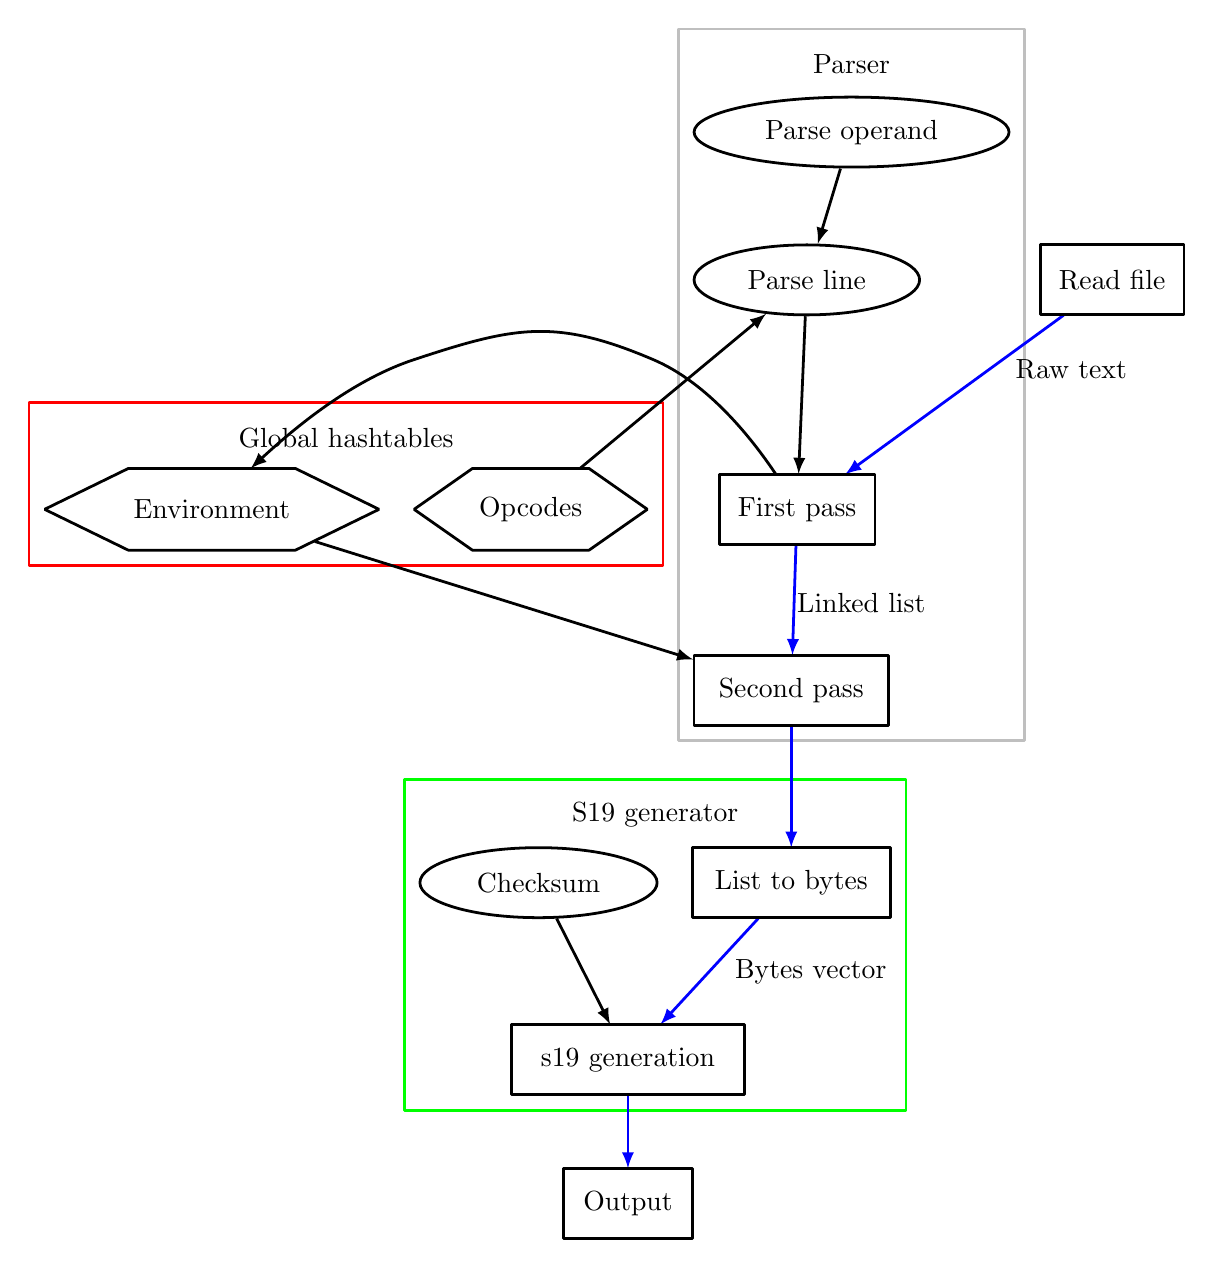
\begin{tikzpicture}[>=latex,line join=bevel,scale=0.7]
  \pgfsetlinewidth{1bp}
%%
\begin{scope}
  \pgfsetstrokecolor{black}
  \definecolor{strokecol}{rgb}{1.0,0.0,0.0};
  \pgfsetstrokecolor{strokecol}
  \draw (8bp,346bp) -- (8bp,430bp) -- (334bp,430bp) -- (334bp,346bp) -- cycle;
  \definecolor{strokecol}{rgb}{0.0,0.0,0.0};
  \pgfsetstrokecolor{strokecol}
  \draw (171bp,412bp) node {Global hashtables};
\end{scope}
\begin{scope}
  \pgfsetstrokecolor{black}
  \definecolor{strokecol}{rgb}{0.75,0.75,0.75};
  \pgfsetstrokecolor{strokecol}
  \draw (342bp,256bp) -- (342bp,622bp) -- (520bp,622bp) -- (520bp,256bp) -- cycle;
  \definecolor{strokecol}{rgb}{0.0,0.0,0.0};
  \pgfsetstrokecolor{strokecol}
  \draw (431bp,604bp) node {Parser};
\end{scope}
\begin{scope}
  \pgfsetstrokecolor{black}
  \definecolor{strokecol}{rgb}{0.0,1.0,0.0};
  \pgfsetstrokecolor{strokecol}
  \draw (201bp,66bp) -- (201bp,236bp) -- (459bp,236bp) -- (459bp,66bp) -- cycle;
  \definecolor{strokecol}{rgb}{0.0,0.0,0.0};
  \pgfsetstrokecolor{strokecol}
  \draw (330bp,218bp) node {S19 generator};
\end{scope}
  \pgfsetcolor{black}
  % Edge: file -> p1
  \pgfsetcolor{blue}
  \draw [->] (540.04bp,474.82bp) .. controls (512.13bp,454.49bp) and (466.82bp,421.48bp)  .. (427.72bp,393.01bp);
  \definecolor{strokecol}{rgb}{0.0,0.0,0.0};
  \pgfsetstrokecolor{strokecol}
  \draw (544bp,447bp) node {Raw text};
  % Edge: po -> pl
  \draw [->] (425.31bp,550.21bp) .. controls (422.67bp,541.47bp) and (419.47bp,530.89bp)  .. (413.62bp,511.57bp);
  % Edge: p1 -> env
  \draw [->] (392.04bp,393.07bp) .. controls (379.48bp,411.84bp) and (356.98bp,440.09bp)  .. (329bp,452bp) .. controls (278.7bp,473.42bp) and (257.91bp,469.13bp)  .. (206bp,452bp) .. controls (176.62bp,442.31bp) and (148.75bp,420.76bp)  .. (121.97bp,396.04bp);
  % Edge: ht -> pl
  \draw [->] (291.36bp,396.07bp) .. controls (316bp,416.55bp) and (353.35bp,447.59bp)  .. (387.05bp,475.59bp);
  % Edge: p1 -> p2
  \pgfsetcolor{blue}
  \draw [->] (402.41bp,356.63bp) .. controls (401.98bp,343.42bp) and (401.4bp,325.37bp)  .. (400.58bp,300.02bp);
  \definecolor{strokecol}{rgb}{0.0,0.0,0.0};
  \pgfsetstrokecolor{strokecol}
  \draw (436bp,327bp) node {Linked list};
  % Edge: chk -> s19
  \draw [->] (279.31bp,164.58bp) .. controls (285.9bp,151.55bp) and (294.85bp,133.85bp)  .. (306.86bp,110.08bp);
  % Edge: v -> s19
  \pgfsetcolor{blue}
  \draw [->] (383bp,164.58bp) .. controls (370.51bp,151.05bp) and (353.38bp,132.49bp)  .. (332.69bp,110.08bp);
  \definecolor{strokecol}{rgb}{0.0,0.0,0.0};
  \pgfsetstrokecolor{strokecol}
  \draw (410bp,137bp) node {Bytes vector};
  % Edge: pl -> p1
  \draw [->] (407.21bp,474.3bp) .. controls (406.4bp,455.2bp) and (405.13bp,425.31bp)  .. (403.77bp,393.22bp);
  % Edge: s19 -> output
  \pgfsetcolor{blue}
  \draw [->] (316bp,73.708bp) .. controls (316bp,65.464bp) and (316bp,55.538bp)  .. (316bp,36.082bp);
  % Edge: env -> p2
  \pgfsetcolor{black}
  \draw [->] (154.93bp,358.48bp) .. controls (206.73bp,342.31bp) and (285.54bp,317.72bp)  .. (349.55bp,297.75bp);
  % Edge: p2 -> v
  \pgfsetcolor{blue}
  \draw [->] (400bp,263.84bp) .. controls (400bp,249.19bp) and (400bp,228.31bp)  .. (400bp,201.04bp);
  % Node: p2
\begin{scope}
  \definecolor{strokecol}{rgb}{0.0,0.0,0.0};
  \pgfsetstrokecolor{strokecol}
  \draw (450bp,300bp) -- (350bp,300bp) -- (350bp,264bp) -- (450bp,264bp) -- cycle;
  \draw (400bp,282bp) node {Second pass};
\end{scope}
  % Node: s19
\begin{scope}
  \definecolor{strokecol}{rgb}{0.0,0.0,0.0};
  \pgfsetstrokecolor{strokecol}
  \draw (376bp,110bp) -- (256bp,110bp) -- (256bp,74bp) -- (376bp,74bp) -- cycle;
  \draw (316bp,92bp) node {s19 generation};
\end{scope}
  % Node: p1
\begin{scope}
  \definecolor{strokecol}{rgb}{0.0,0.0,0.0};
  \pgfsetstrokecolor{strokecol}
  \draw (443bp,393bp) -- (363bp,393bp) -- (363bp,357bp) -- (443bp,357bp) -- cycle;
  \draw (403bp,375bp) node {First pass};
\end{scope}
  % Node: file
\begin{scope}
  \definecolor{strokecol}{rgb}{0.0,0.0,0.0};
  \pgfsetstrokecolor{strokecol}
  \draw (602bp,511bp) -- (528bp,511bp) -- (528bp,475bp) -- (602bp,475bp) -- cycle;
  \draw (565bp,493bp) node {Read file};
\end{scope}
  % Node: chk
\begin{scope}
  \definecolor{strokecol}{rgb}{0.0,0.0,0.0};
  \pgfsetstrokecolor{strokecol}
  \draw (270bp,183bp) ellipse (61bp and 18bp);
  \draw (270bp,183bp) node {Checksum};
\end{scope}
  % Node: ht
\begin{scope}
  \definecolor{strokecol}{rgb}{0.0,0.0,0.0};
  \pgfsetstrokecolor{strokecol}
  \draw (326bp,375bp) -- (296bp,396bp) -- (236bp,396bp) -- (206bp,375bp) -- (236bp,354bp) -- (296bp,354bp) -- cycle;
  \draw (266bp,375bp) node {Opcodes};
\end{scope}
  % Node: env
\begin{scope}
  \definecolor{strokecol}{rgb}{0.0,0.0,0.0};
  \pgfsetstrokecolor{strokecol}
  \draw (188bp,375bp) -- (145bp,396bp) -- (59bp,396bp) -- (16bp,375bp) -- (59bp,354bp) -- (145bp,354bp) -- cycle;
  \draw (102bp,375bp) node {Environment};
\end{scope}
  % Node: v
\begin{scope}
  \definecolor{strokecol}{rgb}{0.0,0.0,0.0};
  \pgfsetstrokecolor{strokecol}
  \draw (451bp,201bp) -- (349bp,201bp) -- (349bp,165bp) -- (451bp,165bp) -- cycle;
  \draw (400bp,183bp) node {List to bytes};
\end{scope}
  % Node: output
\begin{scope}
  \definecolor{strokecol}{rgb}{0.0,0.0,0.0};
  \pgfsetstrokecolor{strokecol}
  \draw (349bp,36bp) -- (283bp,36bp) -- (283bp,0bp) -- (349bp,0bp) -- cycle;
  \draw (316bp,18bp) node {Output};
\end{scope}
  % Node: po
\begin{scope}
  \definecolor{strokecol}{rgb}{0.0,0.0,0.0};
  \pgfsetstrokecolor{strokecol}
  \draw (431bp,569bp) ellipse (81bp and 18bp);
  \draw (431bp,569bp) node {Parse operand};
\end{scope}
  % Node: pl
\begin{scope}
  \definecolor{strokecol}{rgb}{0.0,0.0,0.0};
  \pgfsetstrokecolor{strokecol}
  \draw (408bp,493bp) ellipse (58bp and 18bp);
  \draw (408bp,493bp) node {Parse line};
\end{scope}
%
\end{tikzpicture}



    \newpage
    \section{Source code}
        \subsection{core.h}
            \inputminted{c}{../../src/core.h}
        \subsection{hashtbl.h}
            \inputminted{c}{../../src/hashtbl.h}
        \subsection{instr.h}
            \inputminted{c}{../../src/instr.h}
        \subsection{list.h}
            \inputminted{c}{../../src/list.h}
        \subsection{parser.h}
            \inputminted{c}{../../src/parser.h}
        \subsection{s19.h}
            \inputminted{c}{../../src/s19.h}
        \subsection{utils.h}
            \inputminted{c}{../../src/utils.h}
        \subsection{hashtbl.c}
            \inputminted{c}{../../src/hashtbl.c}
        \subsection{instr.c}
            \inputminted{c}{../../src/instr.c}
        \subsection{list.c}
            \inputminted{c}{../../src/list.c}
        \subsection{main.c}
            \inputminted{c}{../../src/main.c}
        \subsection{parser.c}
            \inputminted{c}{../../src/parser.c}
        \subsection{s19.c}
            \inputminted{c}{../../src/s19.c}
        \subsection{utils.c}
            \inputminted{c}{../../src/utils.c}
        \subsection{opcodes.def}
            \inputminted{c}{../../src/opcodes.def}

\end{document}
